\documentclass[11pt,a4paper,landscape]{article}

\usepackage[left=1.5cm,right=1.5cm,top=1.5cm,bottom=1.5cm]{geometry}
\usepackage{multicol}
\usepackage{graphicx}
\usepackage{amsmath,amssymb}
\usepackage{enumitem}
\setlist[itemize]{noitemsep, topsep=2pt}
\setlist[enumerate]{noitemsep, topsep=2pt}

\setlength{\parindent}{0pt}

\begin{document}
\begin{center}
\textbf{\Huge \uppercase{Algebra Block}}
\vspace{0.2cm}
\hrule
\end{center}
\vspace{0.3cm}

% ==========================================
% CHAPTER 1: INEQUALITIES
% ==========================================
\begin{multicols*}{3}

\textbf{\Huge Inequalities}

\section*{1 Golden Rules}
\begin{itemize}
\item \textbf{Addition / Subtraction:} Adding or subtracting $k$ $\rightarrow$ no change
\item \textbf{Multiplication / Division (+):} Multiply/divide by $+k$ $\rightarrow$ no change
\item \textbf{Multiplication / Division (-):} Multiply/divide by $-k$ $\rightarrow$ flip sign
\item \textbf{Cross Multiplication:} Only if both sides are positive
\end{itemize}

\section*{1.1 Wavy Curve Method (WCM)}

\textbf{Steps:}
\begin{enumerate}
\item \textbf{Built Form:}
$$
\frac{N}{D} > 0 \quad \text{or} \quad \frac{N}{D} < 0
$$

\item \textbf{C.P.:} Roots of numerator and denominator

\item \textbf{Plot:} Number line

\item \textbf{Sign Rule:}
\begin{itemize}
\item Start from right $\rightarrow$ positive
\item Even power $\rightarrow$ no change
\item Odd power $\rightarrow$ sign change
\end{itemize}

\item \textbf{Denominator Rule:}
\begin{itemize}
\item Exclude roots (open intervals)
\item Cancelled factor $\rightarrow$ even $\rightarrow$ no change
\end{itemize}
\end{enumerate}

\vspace{0.2cm}
\begin{center}
  \includegraphics[width=0.9\linewidth]{wavy_curve.jpg}
\end{center}
\vspace{0.2cm}

\section*{1.2 Irrational Equations}

Example:
$$
\sqrt{x+1} - \sqrt{x-1} = \sqrt{4x-1}
$$

\textbf{Steps:}
\begin{enumerate}
\item Square both sides
\item Isolate radicals
\item Square again
\item Check domain: radicands $\ge 0$
\end{enumerate}

\section*{1.3 Irrational Inequalities}

\textbf{Case 1:} $\sqrt{f(x)} > g(x)$

\begin{itemize}
\item $f(x) \ge 0$

\item If $g(x) < 0$:
$$
g(x) < 0 \quad \cap \quad f(x) \ge 0
$$

\item If $g(x) \ge 0$:
$$
g(x) \ge 0 \quad \cap \quad f(x) > [g(x)]^2
$$
\end{itemize}

Final: \textbf{Union}

\textbf{Case 2:} $\sqrt{f(x)} < g(x)$

\begin{itemize}
\item $f(x) \ge 0$, $g(x) > 0$
\item Square and solve
\end{itemize}

Final: \textbf{Intersection}

\section*{1.4 Modulus}

$$
|x|=
\begin{cases}
x & x \ge 0 \\
-x & x < 0
\end{cases}
$$

\textbf{Properties:}
\begin{itemize}
\item $\sqrt{x^2} = |x|$
\item $|ab| = |a||b|$
\item $|a^n| = |a|^n$
\item $\left|\frac{a}{b}\right| = \frac{|a|}{|b|}$
\end{itemize}

\section*{1.5 Modulus Inequalities}

\begin{itemize}
\item $|x| \le \alpha \Rightarrow -\alpha \le x \le \alpha$
\item $|x| \ge \alpha \Rightarrow x \le -\alpha$ or $x \ge \alpha$
\end{itemize}

\section*{1.6 Logarithmic Equations}

\begin{itemize}
\item Variable in power $\rightarrow$ take log
\item Repeating terms $\rightarrow$ substitute
\item Always check domain
\end{itemize}

\section*{1.7 Logarithmic Inequalities}

\textbf{Base $>1$:}
$$
\log_a b \ge c \Rightarrow b \ge a^c
$$

\textbf{$0<a<1$ (flip):}
$$
\log_a b \ge c \Rightarrow b \le a^c
$$

\section*{1.8 Exponential Equations}

$$
f(x) = a^x, \quad a>0,\ a\neq1
$$

\begin{enumerate}
\item $V_2 = 0$
\item $V_1 = 1$
\item $V_1 = -1$ (check power)
\end{enumerate}

\section*{1.9 Exponential Inequalities}

$$
a^x \ge a^y
$$

\begin{itemize}
\item $a>1 \Rightarrow x \ge y$
\item $0<a<1 \Rightarrow x \le y$
\end{itemize}

\end{multicols*}

% ==========================================
% CHAPTER 2: QUADRATIC EQUATIONS
% ==========================================
\newpage
\begin{multicols*}{3}

\textbf{\Huge Quadratic Equations}

\section*{2.1 Basics}
\begin{itemize}
\item $ax^2+bx+c=0 \quad (a\neq0)$
\item \textbf{Form Equation:} $a(x-\alpha)(x-\beta)=0$
\item \textbf{Form Expression:} $y = k(x^2 - (\alpha+\beta)x + \alpha\beta)$
\item \textbf{Roots:} $x = \frac{-b \pm \sqrt{D}}{2a}$, where $D = b^2-4ac$
\end{itemize}

\section*{2.2 Vieta's Formulas}
\textbf{Quadratic ($ax^2+bx+c=0$):}
\begin{itemize}
\item $\alpha+\beta = -\frac{b}{a}$
\item $\alpha\beta = \frac{c}{a}$
\item $|\alpha-\beta| = \frac{\sqrt{D}}{|a|}$
\end{itemize}

\textbf{Higher Degree ($ax^3+bx^2+cx+d=0$):}
\begin{itemize}
\item $\sum \alpha = \alpha+\beta+\gamma = -\frac{b}{a}$
\item $\sum \alpha\beta = \alpha\beta+\beta\gamma+\gamma\alpha = \frac{c}{a}$
\item $\Pi \alpha = \alpha\beta\gamma = -\frac{d}{a}$
\end{itemize}

\section*{2.3 Newton's Formula}
For $ax^2+bx+c=0$ with roots $\alpha, \beta$:
\begin{itemize}
\item Let $S_n = \alpha^n \pm \beta^n$
\item $a(S_n) + b(S_{n-1}) + c(S_{n-2}) = 0$
\item Applicable for higher degrees too.
\item Also use cube roots of unity ($1, \omega, \omega^2$), where $\omega^2+\omega+1=0$ and $\omega^3=1$.
\end{itemize}

\section*{2.4 Nature of Roots}
$D = b^2 - 4ac$
\begin{itemize}
\item $D>0 \Rightarrow$ Real \& Distinct
\item $D=0 \Rightarrow$ Real \& Equal
\item $D<0 \Rightarrow$ Imaginary ($p \pm iq$)
\end{itemize}
\textbf{If $D>0$:}
\begin{itemize}
\item $a,b,c \in \mathbb{Q}$, $D$ is perf. sq. $\Rightarrow$ Roots rational
\item $a,b,c \in \mathbb{Q}$, $D$ not perf. sq. $\Rightarrow$ Conjugate surds ($p \pm \sqrt{q}$)
\item $a,b,c \in \mathbb{Z}$, $a=1$, $D$ is perf. sq. $\Rightarrow$ Roots are integers ($\in \mathbb{Z}$)
\end{itemize}

\section*{2.5 Graphs}
For $y = ax^2+bx+c$:
\begin{itemize}
\item $a>0 \Rightarrow$ Upward parabola ($\cup$)
\item $a<0 \Rightarrow$ Downward parabola ($\cap$)
\item \textbf{Vertex:} $\left(-\frac{b}{2a}, -\frac{D}{4a}\right)$
\item \textbf{Vertex x-coord:} $\frac{\alpha+\beta}{2}$ (Put in eq. for y-axis)
\item $D>0 \Rightarrow$ Cuts x-axis twice
\item $D=0 \Rightarrow$ Touches x-axis
\item $D<0 \Rightarrow$ Does not touch x-axis
\item $c \Rightarrow$ y-intercept
\end{itemize}

\vspace{0.2cm}
\begin{center}
  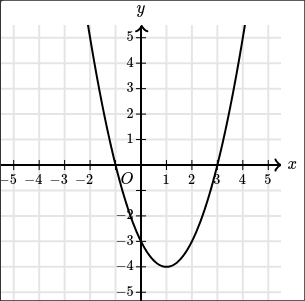
\includegraphics[width=0.9\linewidth]{quadratic_graph.png} \\
  \vspace{0.1cm}
  \small \textit{Graph for $y = x^2 - 2x - 3$}
\end{center}
\vspace{0.2cm}

\section*{2.6 Range of Quadratic}
\begin{itemize}
\item If $a>0 \Rightarrow y \in \left[-\frac{D}{4a}, \infty\right)$
\item If $a<0 \Rightarrow y \in \left(-\infty, -\frac{D}{4a}\right]$
\item If domain restricted, adjust accordingly.
\end{itemize}

\section*{2.7 Range of Rational Functions}
Forms: $\frac{\text{Quad}}{\text{Quad}}, \frac{\text{Lin}}{\text{Quad}}, \frac{\text{Quad}}{\text{Lin}}, \frac{\text{Const}}{\text{Quad}}$
\begin{enumerate}
\item Assume $y$ and cross-multiply as form Quad in $x$.
\item Make $D \ge 0$ (as $x \in \mathbb{R}$).
\item Solve using WCM.
\item \textbf{Check Ans:} Put $x^2$ coeff $= 0$, obtain $y$, put in orig. eq. If you get a valid $x$, keep $y$. If not, remove that $y$.
\end{enumerate}

\section*{2.8 Common Root Conditions}
\begin{itemize}
\item \textbf{Both roots common:}
$$\frac{a_1}{a_2} = \frac{b_1}{b_2} = \frac{c_1}{c_2}$$
\item \textbf{One root common:}
$$(a_1b_2 - a_2b_1)(b_1c_2 - b_2c_1) = (c_1a_2 - c_2a_1)^2$$
Or, put common root in both eqs and solve.
\end{itemize}

\section*{2.9 Location of Roots}
\textbf{Initial Checks:}
\begin{itemize}
\item Always do $a+b+c = ?$ If $0$, root is $1$.
\item For higher degree, use long division.
\item If one root +ve and other -ve, use Vieta's.
\end{itemize}

\textbf{Cases (Assuming $a>0$):}
\begin{itemize}
\item \textbf{Both roots $> k$:}
$$D \ge 0 \quad \cap \quad a \cdot f(k) > 0 \quad \cap \quad k < -\frac{b}{2a}$$
\item \textbf{Both roots $< k$:}
$$D \ge 0 \quad \cap \quad a \cdot f(k) > 0 \quad \cap \quad k > -\frac{b}{2a}$$
\item \textbf{Number $k$ between roots:}
$$a \cdot f(k) < 0$$
\item \textbf{One root between $k_1$ and $k_2$:}
$$f(k_1) \cdot f(k_2) < 0$$
\textit{(Check boundary cases $x=k_1, k_2$ manually)}
\item \textbf{Both roots between $(k_1, k_2)$:}
$$D \ge 0 \cap a \cdot f(k_1) > 0 \cap a \cdot f(k_2) > 0 \cap k_1 < -\frac{b}{2a} < k_2$$
\end{itemize}

\section*{2.10 Transformation of Equation}
Valid for all polynomials.
\begin{itemize}
\item Find eq whose roots are modified (e.g., $\frac{1}{\alpha}, \frac{1}{\beta}$). Let $y = \frac{1}{x} \Rightarrow x = \frac{1}{y}$. Replace $x$ by $\frac{1}{y}$ in original eq.
\item For roots like $\frac{\alpha}{\beta}, \frac{\beta}{\alpha}$, use Vieta's directly.
\end{itemize}

\section*{2.11 Reducible to Quadratic}
\begin{itemize}
\item $ax^3+bx^2+bx+a=0$: Root is usually $1$ or $-1$.
\item $ax^4+bx^3+cx^2+bx+a=0$:
\begin{enumerate}
\item Divide by $x^2$.
\item Group: $a\left(x^2+\frac{1}{x^2}\right) + b\left(x+\frac{1}{x}\right) + c = 0$
\item Sub $t = x+\frac{1}{x} \Rightarrow x^2+\frac{1}{x^2} = t^2-2$.
\item Solve $a(t^2-2) + bt + c = 0$.
\end{enumerate}
\end{itemize}

\end{multicols*}

% ==========================================
% CHAPTER 3: SEQUENCE & SERIES
% ==========================================
\newpage
\begin{multicols*}{3}

\textbf{\Huge Sequence \& Series}

\section*{3.1 Arithmetic Progression (AP)}
\begin{itemize}
\item $a, a+d, a+2d, \dots, a+(n-1)d$
\item $T_n = a + (n-1)d$
\item $S_n = \frac{n}{2}[2a + (n-1)d] = \frac{n}{2}(a + l)$
\item $k^{th}$ from end = $(n-k+1)^{th}$ from start.
\item Adding/Sub/Multiply by constant $\Rightarrow$ still an AP.
\item Common terms b/w two APs $\Rightarrow$ New AP with $D = \text{LCM}(d_1, d_2)$.
\item If $a,b,c \in \text{AP} \Rightarrow 2b = a+c$
\item $a_1 + a_n = a_2 + a_{n-1} = \dots$
\item In linear function of $n$: $S_n = \left(\frac{d}{2}\right)n^2 + \left(a-\frac{d}{2}\right)n + 0$
\item If ratio of $S_n$ is given, find ratio of $n^{th}$ term by replacing $n \rightarrow 2n-1$.
\end{itemize}

\section*{3.2 Arithmetic Mean (AM)}
\begin{itemize}
\item $a, AM, b \Rightarrow AM = \frac{a+b}{2}$
\item Insert $n$ AMs: $a, A_1, A_2, \dots, A_n, b$
\item Total terms $= n+2$
\item $d = \frac{b-a}{n+1}$
\item $m^{th}$ AM $= A_m = a+md$
\item Sum of all $n$ AMs b/w $a$ and $b = n\left(\frac{a+b}{2}\right)$
\end{itemize}

\section*{3.3 Geometric Progression (GP)}
\begin{itemize}
\item $a, ar, ar^2, \dots, ar^{n-1}$
\item $T_n = ar^{n-1}$
\item $S_n = \frac{a(r^n-1)}{r-1}$ for $r>1$, and $\frac{a(1-r^n)}{1-r}$ for $r<1$.
\item $S_\infty = \frac{a}{1-r}$ (if $|r|<1$). If $|r|>1 \Rightarrow S_\infty = \infty$.
\item Reciprocal/multiply/raised to power $\Rightarrow$ still a GP.
\item If $a,b,c \in \text{GP} \Rightarrow b^2 = ac$ (e.g., $1, 2, 4$).
\item $a_1 \cdot a_n = a_2 \cdot a_{n-1} = \dots$
\item If $a_1, a_2 \dots \in \text{GP} \Rightarrow \log a_1, \log a_2 \dots \in \text{AP}$.
\item $a^n + b a^{n-1} + b^2 a^{n-2} + \dots + b^n = \frac{a^{n+1}-b^{n+1}}{a-b}$
\end{itemize}

\section*{3.4 Geometric Mean (GM)}
\begin{itemize}
\item $a, GM, b \Rightarrow GM = \sqrt{ab}$
\item GM of $n$ terms $= (a_1 \cdot a_2 \dots a_n)^{\frac{1}{n}}$
\item Insert $n$ GMs: $a, G_1, G_2, \dots, G_n, b$
\item Common ratio $r = \left(\frac{b}{a}\right)^{\frac{1}{n+1}}$
\item $m^{th}$ GM $= G_m = a r^m$
\item Product of all $n$ GMs b/w $a$ and $b = (\sqrt{ab})^n = (ab)^{n/2}$
\end{itemize}

\section*{3.5 Harmonic Progression (HP)}
\begin{itemize}
\item $a_1, a_2 \dots a_n$ in HP $\Rightarrow \frac{1}{a_1}, \frac{1}{a_2} \dots \frac{1}{a_n}$ in AP.
\item Solve as an AP.
\item $T_n = \frac{1}{a + (n-1)d}$ (using AP's $a$ and $d$).
\item If $a,b,c \in \text{HP} \Rightarrow b = \frac{2ac}{a+c}$.
\end{itemize}

\section*{3.6 Harmonic Mean (HM)}
\begin{itemize}
\item $a, HM, b \Rightarrow HM = \frac{2ab}{a+b}$
\item HM of $n$ terms $= \frac{n}{\frac{1}{a_1} + \frac{1}{a_2} \dots + \frac{1}{a_n}}$
\item Insert $n$ HMs: $a, H_1, H_2 \dots H_n, b$
\item Sum of reciprocals of $n$ HMs $= \sum \frac{1}{H_i} = n\left(\frac{a+b}{2ab}\right)$
\end{itemize}

\section*{3.7 Mean Relations \& Tricks}
\textbf{The Universal Trick:}
$$ \frac{a^{n+1} + b^{n+1}}{a^n + b^n} $$
\begin{itemize}
\item If $n=0 \Rightarrow$ AM
\item If $n=-\frac{1}{2} \Rightarrow$ GM
\item If $n=-1 \Rightarrow$ HM
\end{itemize}

\textbf{Relationship b/w AM, GM, HM:}
\begin{itemize}
\item $A = \frac{a+b}{2}, \quad G = \sqrt{ab}, \quad H = \frac{2ab}{a+b}$
\item $A \ge G \ge H$ (Equality holds if $a=b$)
\item If $A, G, H$ are in GP $\Rightarrow G^2 = AH$.
\item Quadratic eq with roots $a,b$: $x^2 - 2Ax + G^2 = 0$
\item $a, b = A \pm \sqrt{A^2 - G^2}$
\item If $\frac{A}{G} = \frac{m}{n}$, then roots ratio is $\frac{m + \sqrt{m^2-n^2}}{m - \sqrt{m^2-n^2}}$
\end{itemize}

\section*{3.8 Arithmetico-Geometric (AGP)}
\begin{itemize}
\item Form: $a, (a+d)r, (a+2d)r^2, \dots$
\item $T_n = (a+(n-1)d)r^{n-1}$
\item $S_\infty = \frac{a}{1-r} + \frac{dr}{(1-r)^2} \quad (|r|<1)$
\item \textbf{Alternate Method:} Write $S = \dots$, write $rS = \dots$ (shift by 1 term), subtract them, and you are left with a normal GP.
\end{itemize}

\section*{3.9 Properties of Sigma ($\Sigma$)}
\begin{itemize}
\item $\sum (t_r \pm p_r) = \sum t_r \pm \sum p_r$
\item $\sum_{r=1}^n k = nk$
\item $\sum kr = k \sum r$
\item $\sum_{r=a}^b f(r) = \sum_{r=a}^b f(a+b-r)$
\item \textbf{Double Sigma (Symmetric Function):}
$$ \sum_{i=0}^n \sum_{j=0}^n f(i,j) = \sum_{i=0}^n f(i,i) + 2\sum_{i<j} f(i,j) $$
\end{itemize}

\section*{3.10 Important Sums}
\begin{itemize}
\item $\sum r = 1+2+3\dots = \frac{n(n+1)}{2}$
\item $\sum r^2 = 1^2+2^2\dots = \frac{n(n+1)(2n+1)}{6}$
\item $\sum r^3 = 1^3+2^3\dots = \left[\frac{n(n+1)}{2}\right]^2$
\item Sum of first $n$ odd numbers $= n^2$
\item Sum of first $n$ even numbers $= n(n+1)$
\end{itemize}

\end{multicols*}

% ==========================================
% CHAPTER 4: SPECIAL SERIES
% ==========================================
\newpage
\begin{multicols*}{3}

\textbf{\Huge Special Series}

\section*{4.1 Telescopic Series}
\begin{itemize}
\item \textbf{For fractions} (e.g., $\frac{1}{3 \cdot 4 \cdot 5}$): Break into $f(n) - f(n+1)$ using partial fractions.
\item Generally evaluates to: $S_n = \frac{1}{k} \left( \frac{1}{\text{first}} - \frac{1}{\text{last}} \right)$
\item \textbf{For radicals:} Rationalize using conjugate multiply-divide.
  $$ \frac{1}{\sqrt{x+1} + \sqrt{x}} \rightarrow \sqrt{x+1} - \sqrt{x} $$
  Make a difference in the numerator and split so intermediate terms cancel.
\end{itemize}

\section*{4.2 Miscellaneous Series}
\textbf{The Difference Method:}
\begin{enumerate}
\item Write out $T_n$ by observation.
\item If sequence is $4, 11, 21, 34, 50 \dots$ (differences are $7, 10, 13, 16$).
\item If the $1^{st}$ difference forms an \textbf{AP} $\Rightarrow T_n = an^2+bn+c$.
\item If the $1^{st}$ difference forms a \textbf{GP} $\Rightarrow T_n = ar^n+bn+c$.
\item Once $T_n$ is found, use $S_n = \sum T_n$ and simplify using standard $\Sigma$ formulas.
\end{enumerate}

\section*{4.3 Exponential Series}
\begin{itemize}
\item $e^x = \sum_{r=0}^\infty \frac{x^r}{r!} = 1 + \frac{x}{1!} + \frac{x^2}{2!} + \frac{x^3}{3!} \dots \infty$
\item $e^{-x} = \sum_{r=0}^\infty (-1)^r \frac{x^r}{r!} = 1 - \frac{x}{1!} + \frac{x^2}{2!} - \frac{x^3}{3!} \dots \infty$
\item \textbf{Even Powers Only:}
  $$ \frac{e^x + e^{-x}}{2} = 1 + \frac{x^2}{2!} + \frac{x^4}{4!} \dots \infty $$
\item \textbf{Odd Powers Only:}
  $$ \frac{e^x - e^{-x}}{2} = x + \frac{x^3}{3!} + \frac{x^5}{5!} \dots \infty $$
\item \textbf{Simplification Trick:} To evaluate complex sums, remove variables like $n, n^2, n^3$ from the numerator by expanding them to match factorial properties (e.g., $n^2 = n(n-1)+n$). Split fractions until the numerator matches the denominator's factorial base to reduce to standard $e^x$ formats.
\end{itemize}

\section*{4.4 Logarithmic Series}
\begin{itemize}
\item \textbf{Positive Base ($ -1 < x \le 1 $):}
  $$ \ln(1+x) = x - \frac{x^2}{2} + \frac{x^3}{3} - \frac{x^4}{4} + \frac{x^5}{5} \dots \infty $$
\item \textbf{Negative Base ($ -1 \le x < 1 $):}
  $$ \ln(1-x) = -x - \frac{x^2}{2} - \frac{x^3}{3} - \frac{x^4}{4} - \frac{x^5}{5} \dots \infty $$
\end{itemize}

\end{multicols*}

% ==========================================
% CHAPTER 5: PERMUTATIONS & COMBINATIONS
% ==========================================
\newpage
\begin{multicols*}{3}

\textbf{\Huge Permutations \& \\ Combinations}

\section*{1.1 Basic Factorial Notation}
\begin{itemize}
\item $5! = 5 \times 4 \times 3 \times 2 \times 1 = 120$
\item $(-1)! = \text{Not Defined (ND)}$
\item $(a/b)! = \text{Not Defined (ND)}$
\item $0! = 1$
\item $n! = n \times (n-1)!$
\end{itemize}

\section*{1.2 Fundamental Principle of Counting}
\begin{itemize}
\item \textbf{AND (Simultaneously):} If event A happens in $m$ ways and event B happens in $n$ ways, total ways of both happening $\Rightarrow m \times n$.
\item \textbf{OR (Mutually Exclusive):} If event A happens in $m$ ways or event B happens in $n$ ways $\Rightarrow m + n$.
\item \textbf{Slot Rule:} Always fill the slot first that has the strictest rule (e.g., leading zeroes, even numbers, divisibility).
\end{itemize}

\section*{1.3 Theorems of Permutations}
\textbf{Choosing + Arrangement:}
\begin{itemize}
\item Total permutations of $n$ distinct objects, taken \textbf{all} at a time \textbf{with} repetition $\Rightarrow n^n$.
\item Taken \textbf{$r$} at a time \textbf{with} repetition $\Rightarrow n^r$.
\item Taken \textbf{all} without repetition $\Rightarrow n!$.
\item Taken \textbf{$r$} at a time without repetition $\Rightarrow {}^nP_r = \frac{n!}{(n-r)!}$.
\item \textbf{If not distinct:} e.g., arrange $XXXYY \Rightarrow \frac{5!}{3! \times 2!}$.
\end{itemize}

\section*{1.4 Methods of Permutation}
\begin{itemize}
\item \textbf{Tie Method (Always Together):} Tie items together, they act as one unit. 
  $$P_1 [P_2 P_3] P_4 P_5 \Rightarrow 4! \times 2!$$
\item \textbf{GAP Method (Never Together):} Arrange unrestricted items first to create gaps, then fill gaps.
  $$\downarrow P_1 \downarrow P_2 \downarrow P_3 \downarrow P_4 \downarrow P_5 \downarrow$$
  Select 4 gaps for restricted items: $\Rightarrow {}^6P_4 \times 5!$ \quad (or ${}^6C_4 \times 4! \times 5!$)
\item \textbf{Subtraction Method:} Exactly 2 items never together. 
  $$\text{Total Unrestricted} - \text{When Together}$$
  \textit{Note: Only applicable for 2 items. Use PIE instead for $\ge 3$ items.}
\item \textbf{Alternating Method:} 
  $P_1 \downarrow P_2 \downarrow P_3 \downarrow$ \text{ or } $\downarrow P_1 \downarrow P_2 \downarrow P_3$
  $$\Rightarrow 3! \times 3! + 3! \times 3! = 2(3! \times 3!)$$
\end{itemize}

\section*{1.5 Combinations (Only Selecting)}
Order does not matter!
$${}^nC_r = \frac{{}^nP_r}{r!} = \frac{n!}{r!(n-r)!}$$

\textbf{Properties:}
\begin{itemize}
\item ${}^nC_x = {}^nC_y \Rightarrow x=y \text{ OR } x+y=n$
\item ${}^nC_r = {}^nC_{n-r}$
\item ${}^nC_r + {}^nC_{r-1} = {}^{n+1}C_r$
\item ${}^nC_2 = \frac{n(n-1)}{2}, \quad {}^nC_3 = \frac{n(n-1)(n-2)}{6}$
\item ${}^nC_n = 1, \quad {}^nC_0 = 1, \quad {}^nC_{n-1} = n = {}^nC_1$
\end{itemize}

\section*{1.6 Important Results}
\begin{itemize}
\item \textbf{Straight Lines} from $n$ points: ${}^nC_2$
\item \textbf{Triangles} from $n$ points: ${}^nC_3$
\item \textbf{Diagonals} of $n$-sided polygon: ${}^nC_2 - n = \frac{n(n-3)}{2}$
\item \textbf{Intersection of Chords} inside a circle: ${}^nC_4$
\item \textbf{Select Atleast One} from $n$ distinct items: $2^n - 1$
\item \textbf{Handshakes} among $n$ people: ${}^nC_2$
\item \textbf{Gifts Exchanged} (1 person gives to $n-1$): $n(n-1)$
\item \textbf{Total Factors:} If $N = p^a q^b r^c$, 
  $$\text{Factors} = (a+1)(b+1)(c+1)$$
\end{itemize}

\section*{1.7 Groups \& Distribution}
Dividing $n$ distinct items into groups of sizes $a,b,c$:
$$\text{Ways} = \frac{n!}{a! \cdot b! \cdot c!}$$
\textbf{If group sizes are identical:} Divide by the factorial of the number of identical groups.
\begin{itemize}
\item E.g., divide 12 items into groups of $4, 4, 2, 1$:
  $$ \frac{12!}{(4!)^2 \times 2! \times 1!} \times \frac{1}{2!} \quad \text{(as 4 repeats twice)}$$
\end{itemize}
\textbf{Distribution:} If you distribute these groups to $k$ people, multiply by $k!$.
\begin{itemize}
\item E.g., distribute above to 4 children:
  $$ \left( \frac{12!}{(4!)^2 \times 2! \times 1! \times 2!} \right) \times 4! $$
\end{itemize}

\section*{1.8 Principle of Inclusion \& Exclusion (PIE)}
Used to tackle overcounting.
\begin{enumerate}
\item Define Total count usually $(n!)$.
\item Define unwanted conditions ($A, B, C$).
\item Find singles $n(A)$, doubles $n(A \cap B)$, triplets $n(A \cap B \cap C)$.
\end{enumerate}
\textbf{Formula (Pattern: Add singles, sub double, add triple):}
$$\text{Required} = \text{Total} - [\sum n(A) - \sum n(A \cap B) + \sum n(A \cap B \cap C) \dots ]$$

\section*{1.9 Circular Permutation}
\begin{itemize}
\item \textbf{Normal:} Permuting $n$ distinct items in a circle $\Rightarrow (n-1)!$ (The first item can be put anywhere to act as an anchor).
  *E.g., 8 people in 8 chairs $\Rightarrow 7!$*
\item \textbf{Flippable (Garlands \& Necklaces):} As you can rotate/flip them in 3D space and they still have the same arrangement.
  $$\Rightarrow \frac{(n-1)!}{2}$$
\end{itemize}

\section*{2.0 Beggar's Method (Stars and Bars)}
Used for distribution of \textbf{similar/identical} objects to distinct people.
\begin{itemize}
\item \textbf{Equation Form:} $x_1 + x_2 + x_3 \dots + x_r = n$ (where $x \ge 0$)
\item \textbf{Formula:} ${}^{n+r-1}C_{r-1}$
\item \textbf{With Minimum Constraints:} Give the required amount in advance, subtract from total, and solve normally.
  *E.g., 10 coins to 3 beggars ($B_1 \ge 1, B_2 \ge 2, B_3 \ge 3$). Give 1, 2, and 3 in advance. Remaining coins $= 10 - 6 = 4$. Distribute 4 coins to 3 beggars $\Rightarrow {}^{4+3-1}C_{3-1} = {}^6C_2$.*
\item \textbf{Inequality ($\le$):} $x_1 + x_2 \dots \le n$ 
  $\Rightarrow$ Add an extra dummy beggar to absorb the slack and convert to "$=$".
\end{itemize}

\section*{2.1 Legendre's Method}
Finding the exponent of prime number $p$ in $n!$:
$$ E_p(n!) = \left\lfloor \frac{n}{p} \right\rfloor + \left\lfloor \frac{n}{p^2} \right\rfloor + \left\lfloor \frac{n}{p^3} \right\rfloor + \dots $$
\begin{itemize}
\item If finding for a composite number like 10, write $10 = 5 \times 2$. Find the exponent of the \textbf{bottleneck} prime (i.e., the larger prime, 5) and that's your answer.
\end{itemize}

\section*{2.2 Derangement ($D_n$)}
When no item goes into its designated correct spot.
\begin{itemize}
\item $D_1 = 0, \quad D_2 = 1, \quad D_3 = 2, \quad D_4 = 9, \quad D_5 = 44$
\item \textbf{Formula:}
  $$ D_n = n! \left[ \frac{1}{0!} - \frac{1}{1!} + \frac{1}{2!} - \frac{1}{3!} + \dots + \frac{(-1)^n}{n!} \right] $$
\item \textbf{Recursive:} $D_n = (n-1)(D_{n-1} + D_{n-2})$
\item \textbf{Partial Derangement:} Place $r$ items in their correct spots out of $n$ total items:
  $$\Rightarrow {}^nC_r \times D_{n-r}$$
\end{itemize}

\end{multicols*}

% ==========================================
% CHAPTER 5: BINOMIAL THEOREM
% ==========================================
\newpage
\begin{multicols*}{3}

\textbf{\Huge Binomial Theorem}

\section*{5.1 Basics}
\begin{itemize}
\item $(a+b)^n = {}^nC_0 a^n + {}^nC_1 a^{n-1}b^1 + \dots + {}^nC_n b^n$
\item $T_{r+1} = {}^nC_r a^{n-r}b^r$
\item Total terms = $n+1$
\item Sum of all coeff $\Rightarrow (a+b)^n$, put $a=1$ and $b=1$.
\item Compact form = $\sum_{r=0}^n {}^nC_r a^{n-r}b^r$
\item $k^{th}$ term from last = $(n-k+2)^{th}$ from start.
\item $k^{th}$ term from last in $(a+b)^n$ = $k^{th}$ term from starting in $(b+a)^n$.
\item Maximum value of Binomial Coeff is middle term/s. Eg. $({}^{40}C_r \rightarrow \text{max} = {}^{40}C_{20})$
\item \textbf{Numerically Greatest Term} in expansion: Let $m = \frac{n+1}{1 + |\frac{a}{b}|}$. The greatest term is at $m$.
\end{itemize}

\section*{5.2 Binomial Coeff Properties (${}^nC_r$ OR $\binom{n}{r}$)}
\begin{itemize}
\item $\sum_{r=0}^n C_r = 2^n$
\item $C_0 - C_1 + C_2 - C_3 \dots (-1)^n C_n = 0$
\item \textbf{Chain Rule:} ${}^nC_k + {}^{n+1}C_k + {}^{n+2}C_k \dots + {}^{k+n}C_k = {}^{k+n+1}C_{k+1}$
\item $r \cdot {}^nC_r = n \cdot {}^{n-1}C_{r-1}$
\item $\frac{{}^nC_r}{r+1} = \frac{{}^{n+1}C_{r+1}}{n+1}$
\item \textbf{Alternating Sum of Squares:}\\ 
$(C_0)^2 - (C_1)^2 + (C_2)^2 \dots (-1)^n(C_n)^2$
  \begin{itemize}
  \item If $n = \text{odd} \Rightarrow \text{value} = 0$
  \item If $n = \text{even} \Rightarrow \text{value} = (-1)^{n/2} \cdot {}^nC_{n/2}$
  \end{itemize}
\item $C_0 + C_2 + C_4 \dots = C_1 + C_3 + C_5 \dots = 2^{n-1}$
\item $\sum r \cdot {}^nC_r = n 2^{n-1}$
\item $\sum \frac{{}^nC_r}{r+1} = \frac{2^{n+1}-1}{n+1}$
\end{itemize}

\section*{5.3 Product of Coefficients}
\begin{itemize}
\item ${}^nC_0 \cdot {}^nC_n + {}^nC_1 \cdot {}^nC_{n-1} + \dots + {}^nC_n \cdot {}^nC_0 = {}^{2n}C_n$
\item \textbf{Only applicable if:}
  \begin{enumerate}
  \item All terms present.
  \item All terms should be adding (+).
  \item Sum of upper suffix $\rightarrow$ same in each term.
  \item Sum of lower suffix $\rightarrow$ same in each term.
  \end{enumerate}
\end{itemize}

\section*{5.4 Multinomial Theorem}
\begin{itemize}
\item $(a+b+c)^n = \sum \frac{n!}{\alpha! \beta! \gamma!} a^\alpha b^\beta c^\gamma$
\item \textbf{General term:} $\frac{n!}{\alpha! \beta! \gamma!} a^\alpha b^\beta c^\gamma \quad (\alpha+\beta+\gamma = n)$
\item \textbf{No. of terms} in expansion: 
  ${}^{n + \text{var} - 1}C_{\text{var} - 1}$
  \textit{(Only applicable if variables are independent of each other)}
\end{itemize}

\section*{5.5 Applications of Binomial}
\textbf{Divisibility / Remainder:}
\begin{enumerate}
\item Manipulate the Num to become '1' away from a multiple of Den. (Don't forget to split terms if addition/multiplication).
\item Transform the Num to addition/subtraction of that multiple.
\item Check the power of $(-1)$ or $(1)$ and that's your remainder. 
\item For $(-1)$, you add the divisor to it to get the real remainder. Multiply remainder with the excess left when you manipulated the Num.
\item \textbf{Eg:} $\frac{2^{403}}{15} \Rightarrow \frac{(16)^{100} \cdot 2^3}{15} \Rightarrow \frac{(15+1)^{100} \cdot 2^3}{15} \Rightarrow \frac{1 \cdot 8}{15} \Rightarrow 8$.
\end{enumerate}

\textbf{Finding Last Digits:}
\begin{itemize}
\item \textbf{Eg:} Last two digits of $3^{104}$?
\item $(3)^{104} \Rightarrow (9)^{52} \Rightarrow (10-1)^{52}$
\item $= {}^{52}C_0 10^{52} - \dots + {}^{52}C_{50} 10^2(1)^2 - {}^{52}C_{51} 10^1(1)^{51} + 1$
\item $= 10^2(I) - 520 + 1$
\item $= 10^2(I) - 519$ 
\item Last two digits of $-519$ $\Rightarrow 00 - 19 \Rightarrow 81$.
\end{itemize}

\section*{5.6 Integral \& Fractional Part}
\begin{itemize}
\item $R = [R] + f$
\item $R' = \text{conjugate of } R$
\item Sub/add $R$ and $R'$ to remove radical.
\item $R + R' = \text{even} \Rightarrow [R] + f + R' = \text{even}$
\item \textbf{Apply logic:} 
  \begin{itemize}
  \item $f + R' = 1$ (If Adding)
  \item $f - R' = 0$ (If Subtracting)
  \end{itemize}
\end{itemize}

\section*{5.7 Negative \& Fractional Binomial}
For $(a+b)^n$ where $a=1$ \& $|b|<1$, $n \in \text{Negative or Fractional}$.
\begin{itemize}
\item $(1+x)^n = 1 + nx + \frac{n(n-1)}{2!}x^2 + \dots \infty$
\item $(1+x)^{-n} = 1 - nx + \frac{n(n+1)}{2!}x^2 - \dots \infty$
\item $(1-x)^{-n} = 1 + nx + \frac{n(n+1)}{2!}x^2 + \frac{n(n+1)(n+2)}{3!}x^3 + \dots \infty$
\item \textbf{Coeff of $x^r$ in $(1-x)^{-n}$} = ${}^{n+r-1}C_r$ \quad $(n \in \mathbb{N})$
\end{itemize}

\textbf{Important Sequences:}
\begin{itemize}
\item $1 + x + x^2 + x^3 \dots \Rightarrow (1-x)^{-1}$
\item $1 + 2x + 3x^2 + 4x^3 \dots \Rightarrow (1-x)^{-2}$
\item $1 - 2x + 3x^2 - 4x^3 \dots \Rightarrow (1+x)^{-2}$
\end{itemize}

\section*{5.8 Miscellaneous}
\begin{itemize}
\item $C_0 + C_3 + C_6 \dots$ \textbf{[Jumps Questions]}
  \begin{itemize}
  \item If jumps of (3) $\Rightarrow$ put $\omega, \omega^2, 1$ in $(1+x)^n$.
  \end{itemize}
\item \textbf{Approx. Questions:}
  \begin{itemize}
  \item $(1+y)^n \approx (1+ny)$ \quad (If $y$ is very small).
  \end{itemize}
\end{itemize}

\end{multicols*}

\end{document}
